\chapter{Related Work}
\label{Kapitel_erste}
% Labels sind fuer Verknuepfungen im Text notwendig
\textbf{Notice: This template has not yet been fully translated into English. Please contact your supervisor if you have any questions regarding the formatting.}
\bigskip

Kapitel werden mit $\backslash\!chapter\left\{ Titel \right\}$ eingeführt.

Dann folgt das erste Kapitel....

\section{Subchapter}
Ein Unterkapitel wird mit $\backslash\!section\left\{ Titel \right\}$ bezeichnet.

Hier sollen einige weitere Beispiele folgen, wie Bilder, Tabellen und Formeln eingegeben werden.

Tabellen, wie Tabelle \ref{Tabelle_Beispiel} werden wie folgt eingefügt:

\begin{longtable}[c]{L{4cm}C{4cm}p{4cm}}%
	% Definition des Tabellenkopfes
	\caption{Beispiel-Tabelle}
	\label{Tabelle_Beispiel} \\
	\toprule
	\rowcolor{hellgrau}
	1. Spalte	(linksbündig)							&	2. Spalte	(horizontal zentriert)		&		3. Spalte (linksbündig, vertikal zentriert)\\ \midrule
	\endfirsthead % Erster Kopf zu Ende
	%
	% Definition des Tabellenkopfes auf den folgenden Seiten
	\caption*{Beispiel-Tabelle - Fortsetzung}\\
	\toprule
	\rowcolor{hellgrau}
	1. Spalte	(linksbündig)							&	2. Spalte	(horizontal zentriert)		&		3. Spalte (Blocksatz)\\ \midrule
	\endhead % Zweiter Kopf ist zu Ende
	%
	\multicolumn{3}{r}{Fortsetzung von \tab{Tabelle_Beispiel} auf der nächsten Seite}\\
	\endfoot
	\bottomrule
	%\multicolumn{3}{r}{} \\
	\endlastfoot
	% Ab hier folgt der Inhalt der Tabelle
	1. Zeile mit ein bisschen Inhalt zeigt den Unterschied	& Inhalte über mehrere Zeilen zeigen die Effekte & Text über mehrere Zeilen zeigt den Effekt \\ \midrule
	%
	2. Zeile	& Inhalte & Text \\ \midrule
	%
	usw.			& Inhalte & Text 
\end{longtable} 

Ein riesen Vorteil von \LaTeX\; ist die Formelumgebung. Damit diese durchgehend
nummeriert sind, werden diese wie folgt eingefügt, wobei die Gleichung
\begin{align}
	\label{Formel_Beispiel}
	x&=\sqrt[3]{\int \limits_{i=0}^{n} \frac{1}{\sqrt{a^2 + \frac{b^2}{x}}} \mbox{d}x}\\
	a^2+b^2 &= c^2
\end{align}

in den Textfluss eingearbeitet werden sollte. Es ist zu beachten, dass ebenfalls der Bezug zu Formel
\eqref{Formel_Beispiel} im Textfluss lesbar eingefügt sind.

Wenn z.B. das Bild \ref{Bild_Beispiel} eingefügt werden soll, passiert das wie
folgt:
% Bild einfuegen
\begin{figure}[ht!]
	\centering
 	
\includegraphics[width=0.4\textwidth]{LogoFAPS}
	\caption{Unser FAPS-Logo}
	\label{Bild_Beispiel}
\end{figure}

Für einen Eintrag in das Abkürzungsverzeichnis kann bei Verwendung von
Abkürzungen der Befehl $\backslash\!abk\left\{\text{\emph{ABK}}\right\}\left\{ausgeschriebene Bezeichnung\right\}$ verwendet werden. Es sollte
beachtet werden, dass das abzukürzende Wort vor Verwenden der Abkürzung immer
mindestens einmal ausgeschrieben ist.
Das kann dann wie folgt aussehen: Eine zweibuchstabige Abkürzung \abk{ZBA}{zweibuchstabige Abkürzung} ist eine dreibuchstabige Abkürzung \abk{DBA}{dreibuchstabige Abkürzung}.

Für mathematische Konstanten o.ä. funktioniert das auch. Die Gravitationskonstante $\const{g}$ erhält durch
den Befehl $\backslash\!abk\left\{\const{g}\right\}\left\{g\right\}\left\{Gravitationskonstante\right\}$ einen Eintrag im Abkürzungsverzeichnis. Dabei ist die zweite Klammer eine Sortierungshilfe für das Verzeichnis. Die Bezeichnung in der dritten Klammer kann für das Verzeichnis angepasst werden und erscheint nicht im Text. Ausgeführt sieht das dann so aus: \abk{$\const{g}$}{g}{Gravitationskonstante}. Auch griechische Buchstaben sind kein Problem, wie beispielsweise der \abk{$\eta$}{eta}{Wirkungsgrad} mit $\backslash\!abk\left\{\eta\right\}\left\{eta\right\}\left\{Wirkungsgrad\right\}$ beschrieben wird.

Im Literaturverzeichnis sind alle Quellen anzugeben. Des Weiteren kann darin für weitere Informationen geschmökert werden.
Zitieren funktioniert mit dem Befehl $\backslash\!cite\left\{ Buch\;etc.\right\}$. Das ergibt dann z.B. \cite{Resetarics.2009}. Die Literaturliste kann als BiBTeX-Datei aus Citavi exportiert werden. Dabei tauchen dann im Text nur die Quellen auf, welche auch tatsächlich zitiert wurden.

\subsection{Sub-subchapter}
In einer Arbeit sollten die Kapitel und Abschnitte nicht tiefer als die dritte
Ebene sein. Zumindest tauchen weitere Überschriften nicht im Inhaltsverzeichnis auf.

Als Ergänzung wird im Folgenden noch aufgezeigt, wie zwei Bilder nebeneinander
dargestellt werden. Referenziert werden diese Bilder analog zu vorher. Beispielsweise zeigt Abbildung \ref{Bild_Beispiel_zwei_Bilder_links} eine Roboterhand mit einem Apfel, wobei in Abbildung \ref{Bild_Beispiel_zwei_Bilder_rechts} wiedermal das FAPS-Logo zu sehen ist. Zu beachten ist, dass nur die Hauptbeschriftung im Abbildungsverzeichnis auftaucht. Diese ist oft auch einfach nur eine Kurzform.

\begin{figure}[ht!]

% Breite darf maximal 0.49*\textwidth sein, wobei die Hoehe der zwei Bilder
% gleich sein sollte
\newcommand{\pictureheight}{5cm}

	\begin{minipage}[c]{.49\textwidth}
		\centering
		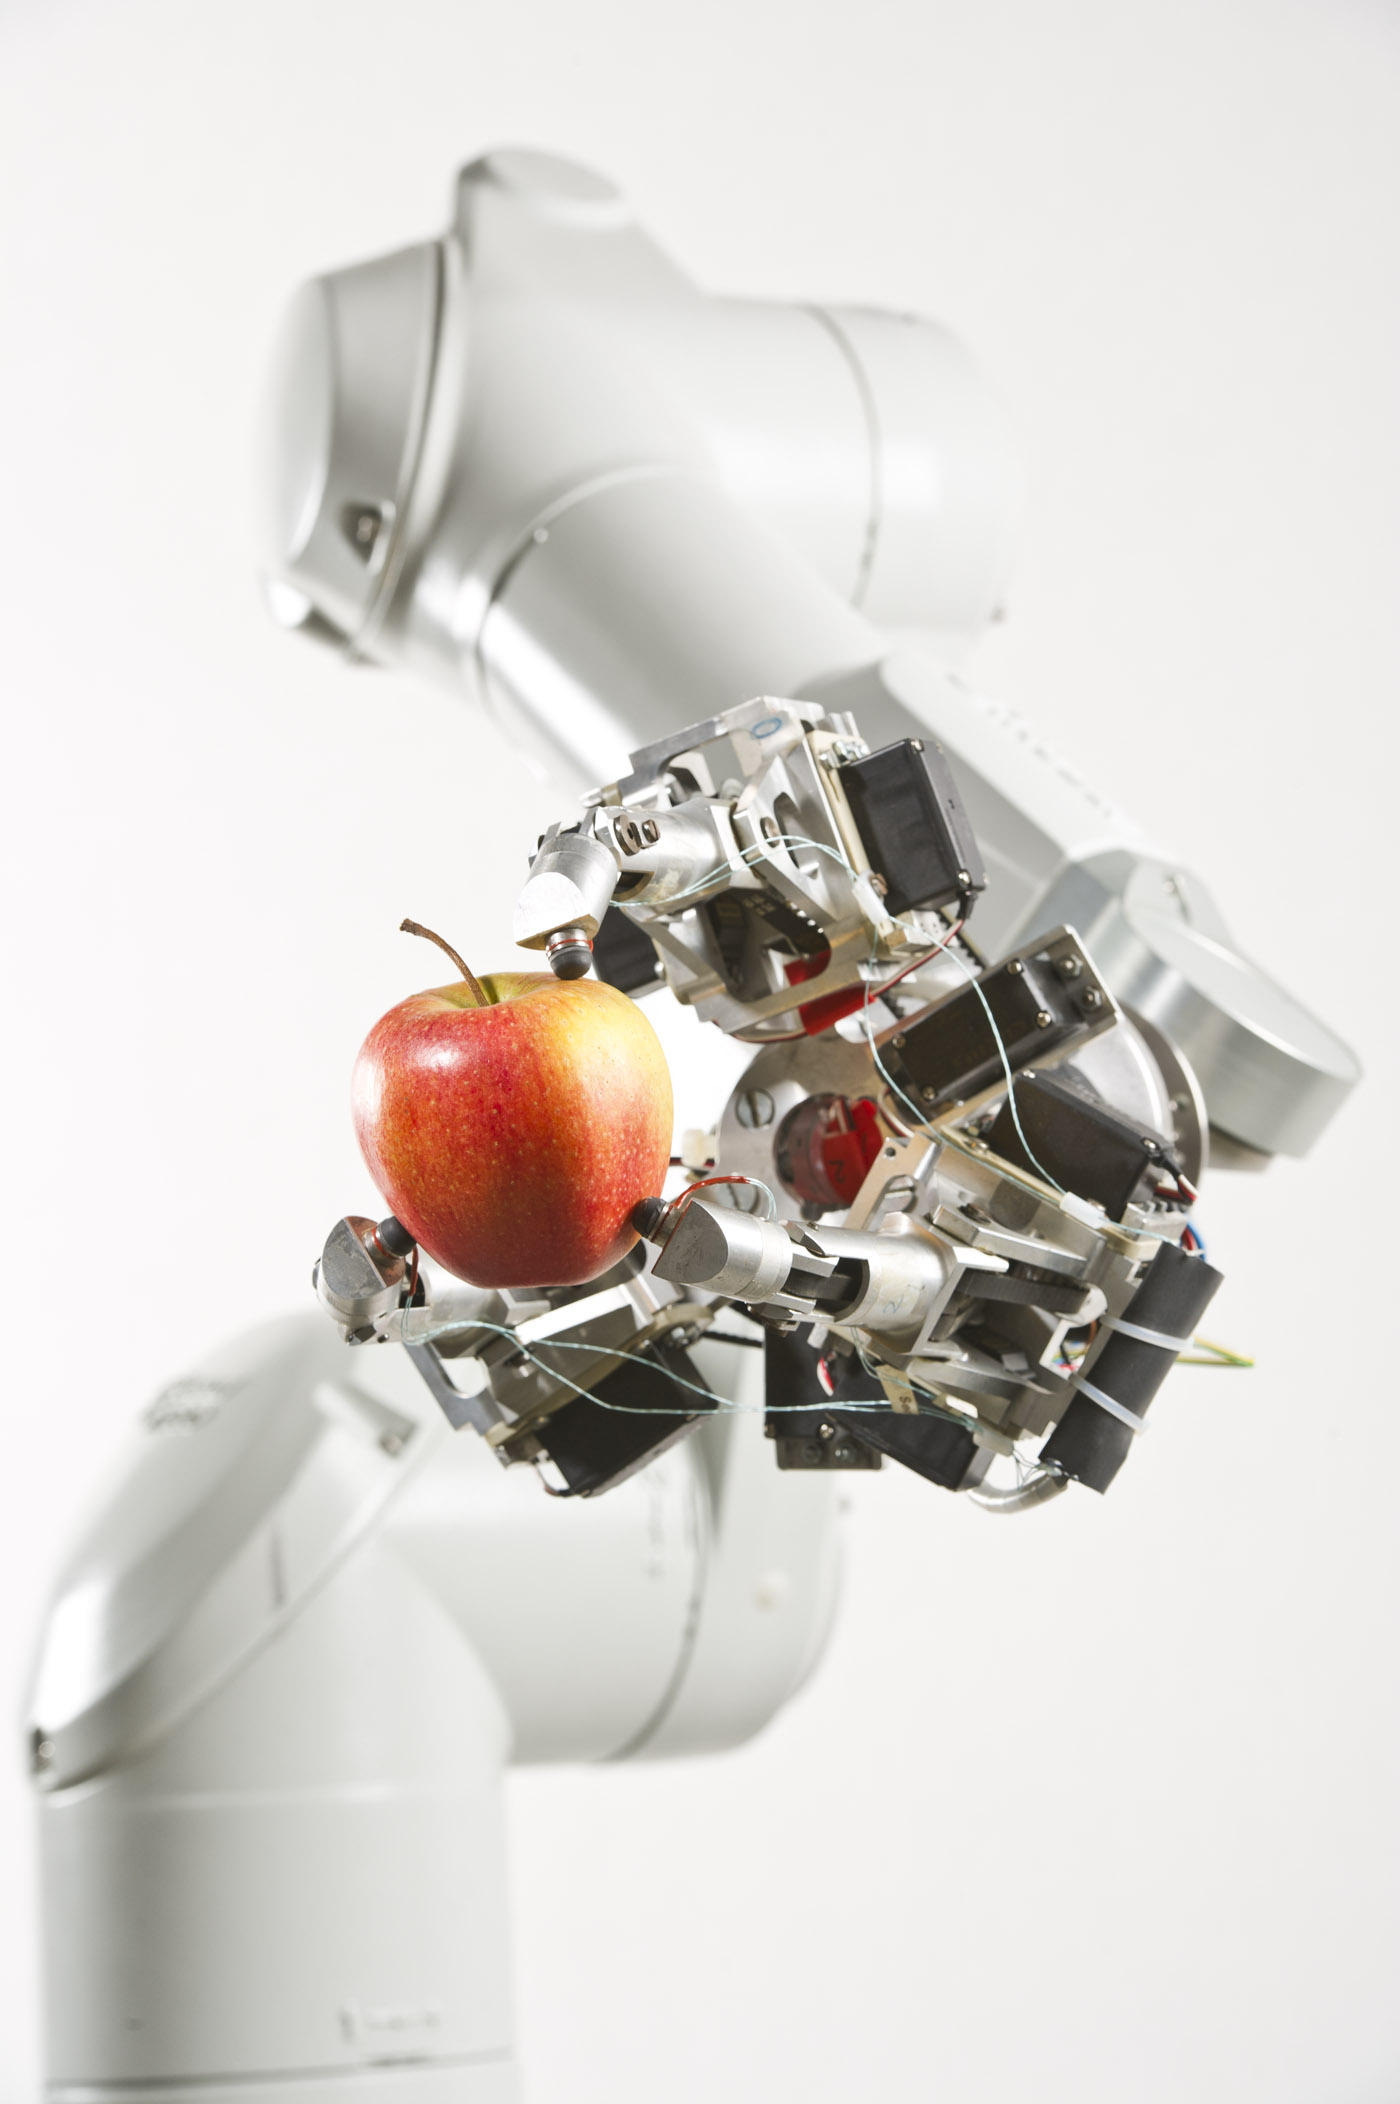
\includegraphics[height=\pictureheight]{Biomechgreifer.jpg}
		\subcaption{Roboterhand mit Apfel}
		\label{Bild_Beispiel_zwei_Bilder_links}
	\end{minipage}
%	
	\begin{minipage}[c]{.49\textwidth}
        \centering
		
\includegraphics[height=\pictureheight]{LogoFAPS}
		\subcaption{FAPS-Logo}
		\label{Bild_Beispiel_zwei_Bilder_rechts}
	\end{minipage}
    	
    	\caption[Zwei Bilder nebeneinander]{Hier sind zwei Bilder zu sehen, welche nebeneinander angeordnet sind.}
	\label{Bild_Beispiel_zwei_Bilder}

\end{figure}

Auflistungen werden wie folgt gemacht:
\begin{itemize}
	\item Das wird der erste Stichpunkt
	\item Ein zweiter Stichpunkt
	
	\begin{itemize}
		\item Das ist die nächste Ebene
	\end{itemize}
	
\end{itemize}